\documentclass[../../Thesis.tex]{subfiles}
\usepackage[italian]{babel}

\begin{document}
\chapter{Metodologia}
Questa sezione descrive in dettaglio l'approccio seguito per affrontare il problema della classificazione degli smart contracts. Questo capitolo è fondamentale per comprendere come sono stati raccolti, pre-processati e utilizzati i dati, come è sono stati configurati e addestrati i modelli e quali strumenti e tecniche sono stati impiegati per ottenere i risultati presentati.

La metodologia adottata in questa tesi è suddivisa nelle seguenti fasi principali:
\begin{enumerate}
    \item Raccolta e preparazione dei dati: esplorazione del dataset utilizzato, delle tecniche di pre-processing applicate e delle modalità di suddivisione dei dati per l'addestramento e la valutazione.
    \item Modellazione: descrizione dell'architettura dei modelli utilizzati, delle scelte di configurazione e delle strategie di addestramento.
.
\end{enumerate}
Ogni fase sarà trattata in modo dettagliato, evidenziando le scelte metodologiche compiute e le motivazioni alla base di tali scelte. Questo approccio sistematico garantisce trasparenza e replicabilità del lavoro svolto, consentendo ad altri  di comprendere e, eventualmente, replicare i risultati ottenuti.
    
\section{Esplorazione dei dati}
Il dataset \cite{rossini2022slitherauditedcontracts} utilizzato in questo progetto è un dataset disponibile pubblicamente sulla piattaforma HuggingFace una delle più importanti piattaforme per il Natural Language Processing. HF è un'infrastruttura open-source che fornisce accesso a una vasta gamma di modelli di deep learning pre-addestrati, tra cui alcuni dei più avanzati nel campo del NLP.
Questo dataset contiene informazioni su 106.474 SmartContracts pubblicati sulla rete Ethereum. Ogni elemento nel dataset è composto da quattro elementi:
\begin{itemize}
    \item  \textbf{Address}: l'indirizzo del contratto
    \item  \textbf{SourceCode}: il codice sorgente del contratto, scritto in linguaggio Solidity
    \item  \textbf{ByteCode}: il codice bytecode del contratto, ottenuto a partire dalla compilazione del codice sorgente utilizzando il compilatore di Solidity. Questo bytecode è quello che viene eseguito sulla macchina virtuale di Ethereum (EVM).
    \item  \textbf{Slither}: il risultato dell'analisi statica del contratto con Slither, un tool open-source per l'analisi statica di contratti scritti in Solidity. Questo risultato è un array di valori che vanno da 1 a 5, dove ogni numero  rappresenta la presenza di una vulnerabilità e 4 rappresenta un contratto safe, cioè privo di vulnerabilità.
\end{itemize}
Le vulnerabilità che sono state prese in questo lavoro sono le seguenti:
\begin{itemize}
    \item Access-Control
    \item Arithmetic
    \item Other
    \item Reentrancy
    \item Safe
    \item Unchecked-Calls
\end{itemize}
Prima della costruzione dei modelli è stata affrontata una fase di analisi esplorativa dei dati. Questa fase è stata svolta per comprendere meglio la struttura del dataset e dei contratti da classificare, per individuare eventuali problemi. A livello pratico, questa fase di analisi esplorativa dei dati è stata eseguita utilizzando il linguaggio Python, con l'ausilio di librerie come Pandas, NumPy, Matplotlib e Seaborn per l'analisi e la visualizzazione dei dati.
Il dataset è diviso in tre sottoinsiemi: training, validation e test set.
Il dataset di training è composto da 79.641 contratti, il dataset di validazione da 10.861 contratti e il dataset di test da 15.972 contratti.
Tutte le informazioni sono presenti per tutti i contratti tranne l'informazione relativa al bytecode, che risulta essere assente per pochissimi contratti come visibile nella Tabella \ref{tab:no_bytecode_count}. 
\begin{table}[h!]
    \centering
    \begin{tabular}{|l|c|c|}
        \hline
        \textbf{Dataset} & \textbf{Count} & \textbf{\%} \\
        \hline
        Train & 227 & 0.285\% \\
        Test & 51 & 0.319\% \\
        Validation & 30 & 0.276\% \\
        \hline
    \end{tabular}
    \caption{Conteggio e Percentuale di Contratti Senza Bytecode per Dataset}
    \label{tab:no_bytecode_count}
\end{table}
Per ottenere una visione d'insieme delle lunghezze dei contratti, abbiamo calcolato la lunghezza media del source code e del bytecode. Prima del preprocessing le lunghezze medie di SourceCode e ByteCode sono rispettivamente di 3155 token e 8114 token.
Abbiamo visualizzato la distribuzione delle lunghezze del source code utilizzando un istogramma. Per migliorare la leggibilità del grafico, abbiamo raggruppato i dati per quanto riguarda il source code in intervalli di 500 token. L'istogramma è accompagnato da una linea che indica la lunghezza media dei token rappresentata con una linea tratteggiata rossa.

L'inclusione delle lunghezze medie fornisce un punto di riferimento utile per interpretare le distribuzioni e confrontare i singoli esempi di codice rispetto alla media del dataset. Queste analisi sono fondamentali per le successive fasi di preprocessing e modellazione, garantendo che i modelli possano gestire efficacemente la variabilità presente nei dati.
Sul bytecode non è stato applicato nessun tipo di preprocessing per ridurre la dimensione dei dati. Per quanto riguarda il codice sorgente sono stati eliminati tutti i commenti e le funzioni getter monoistruzione, cioè tutte quelle funzioni \texttt{getX()} le quali abbiano come unica istruzione una istruzione di return, poichè sono state assunte come funzioni corrette, l'eliminazione di queste stringhe è avvenuta tramite una ricerca delle stringhe effettuata con una regex.
Abbiamo unito i set di dati di addestramento, test e validazione in un unico DataFrame per analizzare le lunghezze del source code e del bytecode. In particolare, sono state calcolate rispettivamente le lunghezze del codice sorgente e del bytecode. Effettuando le rimozioni dei commenti la media del numero di token del sourcecode scende a 1511 token, mostrando come la rimozione dei commenti abbia un grande impatto sulla lunghezza media del codice. Rimuovendo anche le funzioni getter monoistruzione la lunghezza media del source code scende a 1481 token.
\begin{figure}[htbp]
    \centering
    \begin{subfigure}[b]{0.49\textwidth}
        \centering
        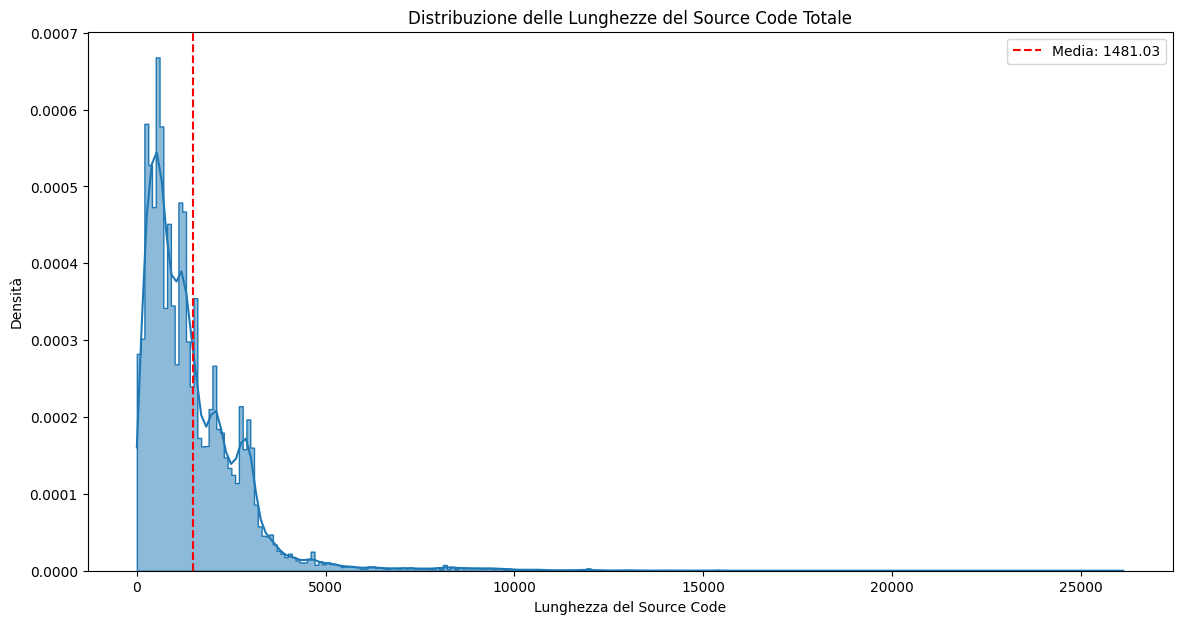
\includegraphics[width=\textwidth]{../../img/SCTokensPreprocessed.png}
        \caption{Distribuzione delle Lunghezze del Source Code dopo il preprocessing}
        \label{fig:sourcecode_length_distribution}
    \end{subfigure}
    \hfill
    \begin{subfigure}[b]{0.49\textwidth}
        \centering
        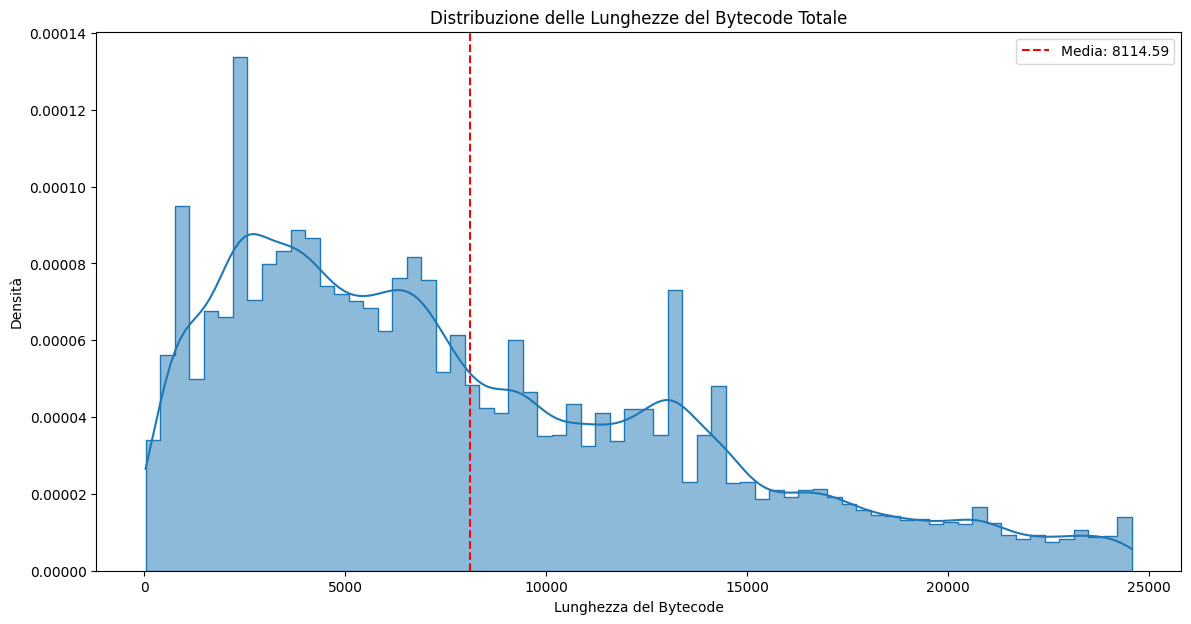
\includegraphics[width=\textwidth]{../../img/BCTokensPreprocessed.png}
        \caption{Distribuzione delle Lunghezze del Bytecode dopo il preprocessing}
        \label{fig:bytecode_length_distribution}
    \end{subfigure}
    \caption{Distribuzioni delle lunghezze del source code e del bytecode.}
    \label{fig:length_distributions}
\end{figure}
Poichè successivamente andremo a classificare i contratti con dei modelli nella famiglia BERT che prendono in input sequenze di token lunghe al massimo 512 token abbiamo calcolato la percentuale di contratti che non superano questa soglia e in alcuni suoi multipli, per capire quanti contratti riusciamo a classificare per intero e quanti verranno troncati. I risultati sono mostrati nella Tabella \ref{tab:summary}.
\begin{table}[h!]
    \centering
    \begin{tabular}{|l|c|c|c|c|}
        \hline
        \textbf{Metrica} & \textbf{Sotto 512} & \textbf{Sotto 1024} & \textbf{Sotto 1536} & \textbf{Media} \\
        \hline
        \textbf{Source Code (\%)} & 21.90 & 46.04 & 64.77 & 62.21 \\
        \textbf{Bytecode (\%)} & 1.56 & 6.31 & 8.75 & 58.69 \\
        \hline
    \end{tabular}
    \caption{Percentuale di contratti sotto varie lunghezze in token.}
    \label{tab:summary}
\end{table}


Diventa però importante notare, che per molti casi di contratti che superano i 5000 token questi sono così lunghi poichè riportano in calce al contratto anche il codice sorgente di librerie esterne, che non è di interesse per la classificazione delle vulnerabilità. 


\subsection{Distribuzione delle Classi e Matrici di Co-occorrenza}
Successivamente, la fase di esplorazione dei dati ha previsto l'analisi delle classi di vulnerabilità dei dati. In questa sezione, presentiamo la distribuzione delle classi e le matrici di co-occorrenza per i dataset di addestramento, test e validazione. Si precisa che i risultati di seguito proposti si riferiscono già al dataset da cui sono stati sottratti i contratti privi di bytecode.

\subsubsection{Distribuzione delle Classi}

La Tabella \ref{tab:class_distribution} mostra la distribuzione delle classi per i tre dataset. È evidente che la classe 'unchecked-calls' è la più frequente in tutti e tre i dataset, mentre la classe 'access-control' è la meno rappresentata.
\begin{table}[h!]
    \centering
    \begin{tabular}{|l|c|c|c|c|c|c|c|c|}
        \hline
        \textbf{Class} & \multicolumn{2}{|c|}{\textbf{Train}} & \multicolumn{2}{|c|}{\textbf{Test}} & \multicolumn{2}{|c|}{\textbf{Validation}} & \multicolumn{2}{|c|}{\textbf{Full}} \\
        \cline{2-9}
        & \textbf{Count} & \textbf{\%} & \textbf{Count} & \textbf{\%} & \textbf{Count} & \textbf{\%} & \textbf{Count} & \textbf{\%} \\
        \hline
        access-control & 11619 & 8.71\% & 2331 & 8.71\% & 1588 & 8.73\% & 15538 & 8.72\% \\
        arithmetic & 13472 & 10.10\% & 2708 & 10.12\% & 1835 & 10.09\% & 18015 & 10.10\% \\
        other & 20893 & 15.67\% & 4193 & 15.67\% & 2854 & 15.69\% & 27940 & 15.67\% \\
        reentrancy & 24099 & 18.07\% & 4838 & 18.09\% & 3289 & 18.08\% & 32226 & 18.08\% \\
        safe & 26979 & 20.23\% & 5405 & 20.20\% & 3676 & 20.21\% & 36060 & 20.23\% \\
        unchecked-calls & 36278 & 27.21\% & 7276 & 27.20\% & 4951 & 27.21\% & 48505 & 27.21\% \\
        \hline
    \end{tabular}
    \caption{Distribuzione delle Classi nei Dataset di Addestramento, Test, Validazione e Completo}
    \label{tab:class_distribution}
\end{table}

Le Figure \ref{fig:relative_distribution} e \ref{fig:absolute_distribution} mostrano rispettivamente la distribuzione percentuale e assoluta delle classi nell'intero dataset. Queste visualizzazioni forniscono una panoramica chiara della frequenza delle diverse classi all'interno del dataset, evidenziando le differenze di distribuzione tra le classi.
\begin{figure}[h!]
    \centering
    \begin{subfigure}[b]{0.45\linewidth}
      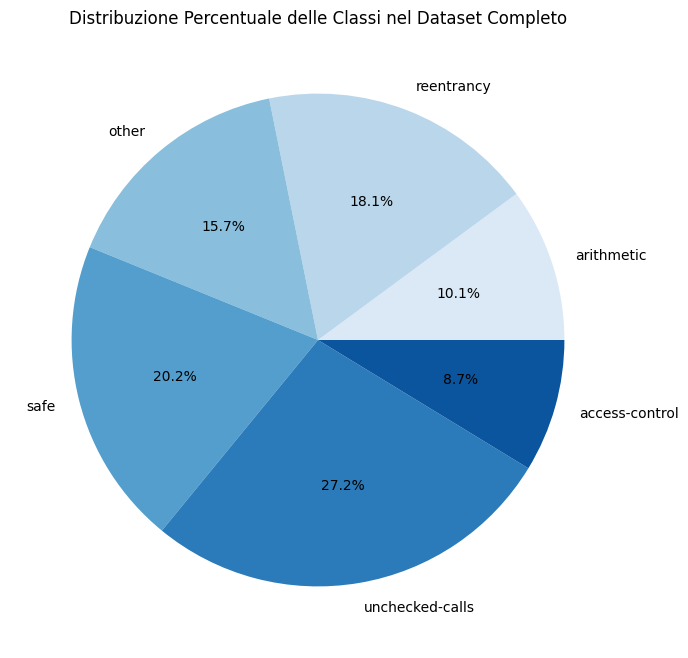
\includegraphics[width=\linewidth]{../../img/class-distribution-relative.png}
      \caption{Distribuzione Percentuale delle Classi}
      \label{fig:relative_distribution}
    \end{subfigure}
    \hspace{0.5cm}
    \begin{subfigure}[b]{0.45\linewidth}
      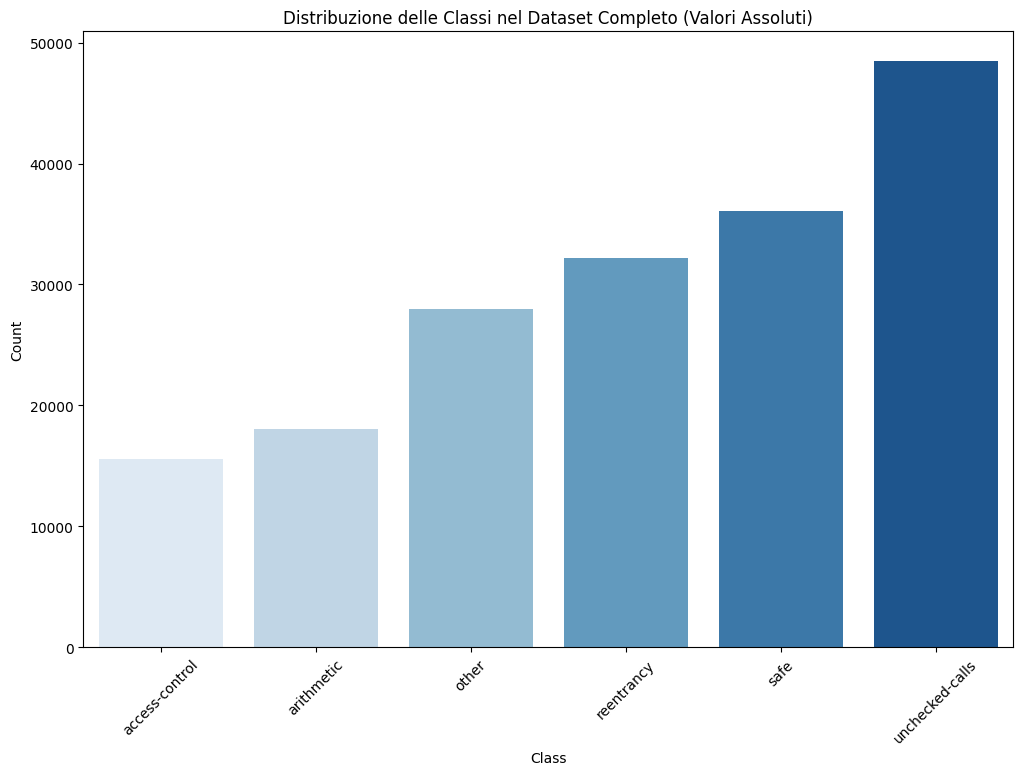
\includegraphics[width=\linewidth]{../../img/class-distribution-absolute.png}
      \caption{Distribuzione Assoluta delle Classi}
      \label{fig:absolute_distribution}
    \end{subfigure}
    \caption{Distribuzioni delle Classi nell'intero dataset, in termini relativi e assoluti.}
    \label{fig:class_distributions}
  \end{figure}
  Dalla distribuzione delle classi nei diversi dataset, possiamo osservare che:

  \begin{itemize}
      \item Le classi sono distribuite in modo abbastanza uniforme nei dataset di addestramento, test e validazione, con percentuali simili tra i tre split per classe
      \item La classe 'unchecked-calls' è la più frequente in tutti e tre i dataset, con una presenza significativa soprattutto nel dataset di addestramento (36278 occorrenze).
      \item La classe 'access-control' è la meno frequente, con il numero più basso di occorrenze nel dataset di validazione (1588 occorrenze).
      \item Le classi 'safe' e 'reentrancy' sono anche abbastanza rappresentate
  \end{itemize}
\subsubsection{Matrici di Co-occorrenza}
Le Tabelle \ref{fig:train_cooccurrence_matrix}, \ref{fig:test_cooccurrence_matrix} e \ref{fig:val_cooccurrence_matrix} mostrano le matrici di co-occorrenza per i dataset di addestramento, test e validazione rispettivamente. Le matrici di co-occorrenza indicano la frequenza con cui ogni coppia di classi appare insieme nello stesso elemento.

In questa sezione, vengono presentate le matrici di co-occorrenza per ogni split del dataset, mostrando sia in termini assoluti che relativi il numero di cooccorrenze tra le varie classi.

\begin{figure}[H]
    \centering
    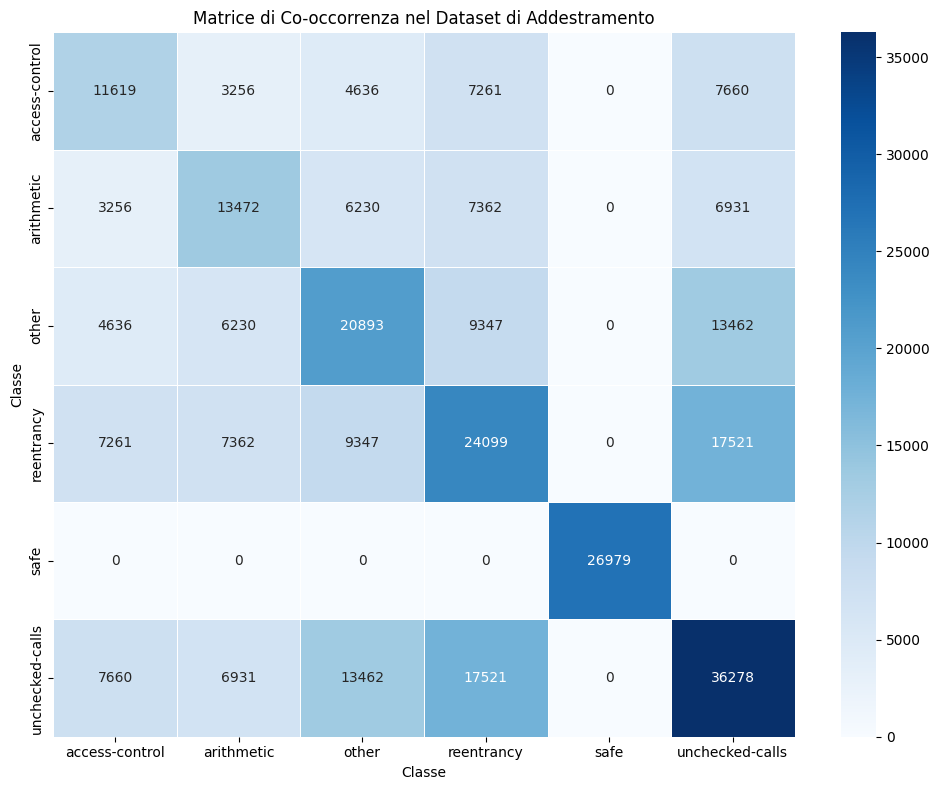
\includegraphics[width=0.7\textwidth]{../../img/TrainCo-occurrency.png}
    \caption{Matrice di Co-occorrenza nel Dataset di Addestramento}
    \label{fig:train_cooccurrence_matrix}
\end{figure}

\begin{figure}[H]
    \centering
    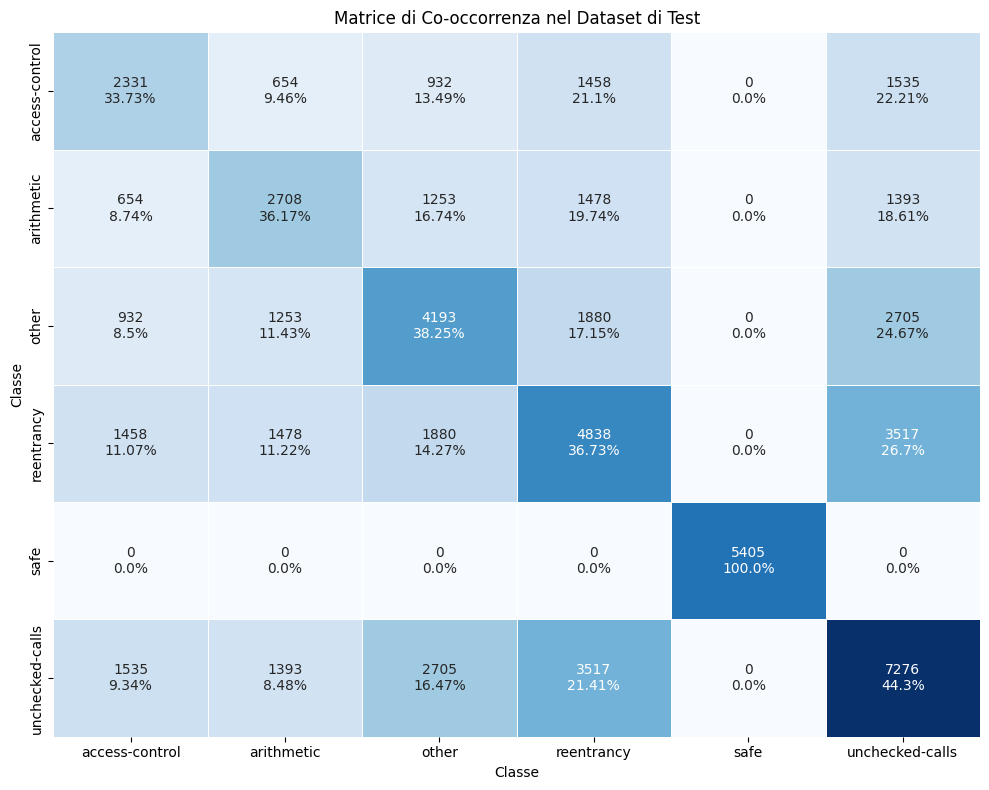
\includegraphics[width=0.7\textwidth]{../../img/TestCo-occurrency.png}
    \caption{Matrice di Co-occorrenza nel Dataset di Test}
    \label{fig:test_cooccurrence_matrix}
\end{figure}

\begin{figure}[h]
    \centering
    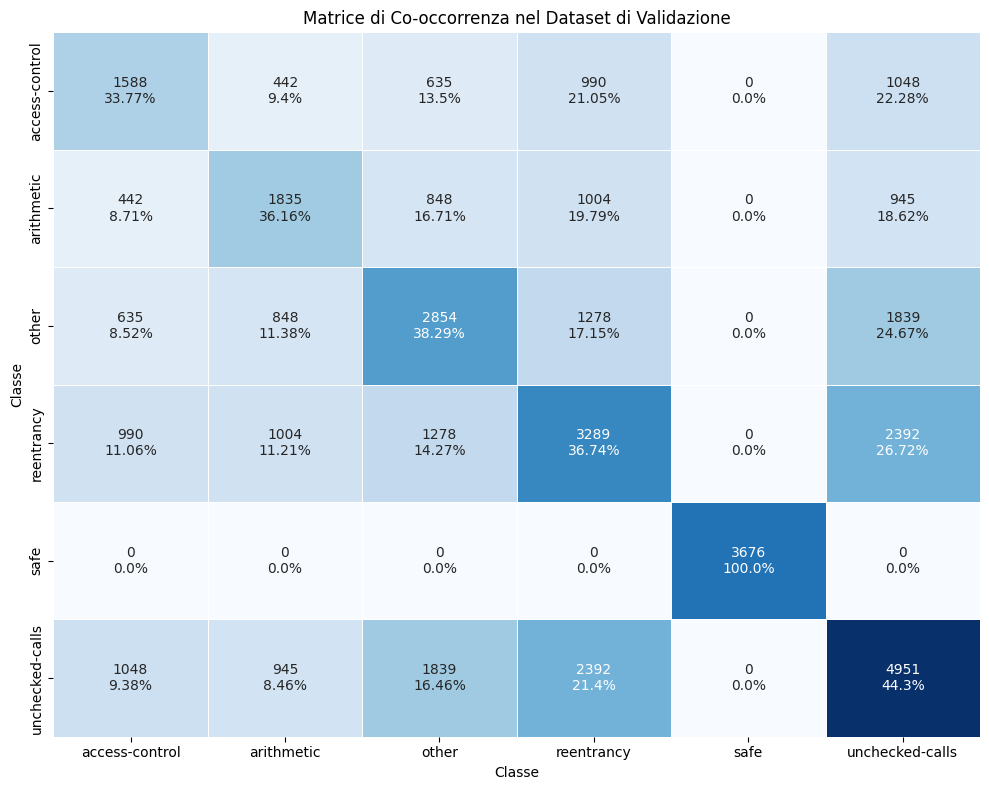
\includegraphics[width=0.7\textwidth]{../../img/ValCo-occurrency.png}
    \caption{Matrice di Co-occorrenza nel Dataset di Validazione}
    \label{fig:val_cooccurrence_matrix}
\end{figure}



Analizzando le matrici di co-occorrenza, notiamo che:

\begin{itemize}
    \item La classe safe, che rappresenta i contratti privi di vulnerabilità, correttamente non apparte contemporaneamente a nessuna delle altre classi. 
    \item Le classi 'unchecked-calls' co-occorrono frequentemente con 'reentrancy', 'other', e 'access-control'. Questo suggerisce che i contratti con chiamate non verificate spesso presentano anche altri tipi di vulnerabilità.
    \item Le classi 'arithmetic' e 'reentrancy' mostrano una co-occorrenza significativa, suggerendo che le vulnerabilità aritmetiche possono spesso essere associate a problemi di rientro.
\end{itemize}

Questi risultati evidenziano l'importanza di considerare la co-occorrenza delle classi quando si analizzano le vulnerabilità nei contratti intelligenti, poiché molte vulnerabilità non si verificano in isolamento ma tendono a manifestarsi insieme ad altre.


\section{Modellazione}
In questa sezione, descriviamo l'architettura dei modelli utilizzati per la classificazione dei contratti intelligenti. In particolare, presentiamo i dettagli relativi ai modelli BERT utilizzati, alle scelte di configurazione e alle strategie di addestramento.
Come si evince dalla sezione precente le feature su cui i modelli dovranno basare le loro predizioni sono il codice sorgente e il bytecode dei contratti, cioè dati di natura testuale. La natura dei dati fa sì che problema possa essere affrontato efficacemente utilizzando tecniche di elaborazione del linguaggio naturale (NLP, Natural Language Processing).

\subsection{Natural Language Processing, NLP}
L'Elaborazione del Linguaggio Naturale (NLP, da \emph{Natural Language Processing}) è un campo  di studi interdisciplinare che combina linguistica, informatica e intelligenza artificiale. Si occupa dell'interazione tra computer e linguaggio umano (naturale), in particolare del processamento, analisi e costruzione di modelli riguardanti grandi quantità di dati linguistici naturali \cite{jurafsky2009speech}. 
Le due grandi sfide dell'NLP si possono riassumere in due grandi aree di ricerca: la comprensione del linguaggio e la generazione del linguaggio. La comprensione del linguaggio comprende compiti come l'analisi sintattica, l'analisi semantica, il riconoscimento delle entità nominate e la risoluzione delle coreferenze. Questi compiti sono cruciali per la conversione del linguaggio naturale in una rappresentazione formale che le macchine possano elaborare. L'analisi sintattica, ad esempio, mira a determinare la struttura grammaticale di una frase, mentre l'analisi semantica si concentra sulla comprensione del significato del testo. In secondo luogo 
la generazione del linguaggio riguarda la produzione automatica di testo, che può includere la sintesi vocale, la traduzione automatica e la generazione di risposte automatiche in chatbot. Questo aspetto dell'NLP è fondamentale per creare sistemi che non solo comprendano il linguaggio umano, ma che possano anche comunicare in modo naturale e coerente con gli utenti.

Negli ultimi  anni, il campo dell'NLP ha fatto enormi progressi passando dall'epoca delle schede perforate e dell'elaborazione batch (in cui l'analisi di una frase poteva richiedere fino a 7 minuti) all'era di Google e simili (in cui milioni di pagine web possono essere elaborate in meno di un secondo) \cite{6786458}, sino ad arrivare ai giorni d'oggi con l'avvento di modelli di deep learning. Per decenni, l'approccio alla ricerca nel campo dell'NLP prevedeva l'utilizzo di modelli shallow come SVM \cite{SVM} e regressione logistica allenati su feature sparse e fortemente multidimensionali. Negli ultimi anni, d'altro canto,  le reti neurali basati su rappresentazioni di vettori densi hanno prodotto risultati superiori su una grande vastità di task diversi nel mondo dell'NLP \cite{TrendsInNLP}. 
Lo stato dell'arte attuale nell'NLP è in molti task rappresentato dall'introduzione di una nuova architettura, che è andata a sostituire i modelli RNN e LSTM \cite{LSTM} tradizionali, ovvero i modelli basati su Trasformer, introdotti per la prima volta nel paper "Attention is All You Need" da Vaswani et al. nel 2017 \cite{AttentionIsAllYouNeed}. I Transformer hanno rivoluzionato il campo grazie al meccanismo di self-attention, che consente al modello di valutare e ponderare l'importanza di ogni parola in una frase rispetto alle altre parole della stessa frase, indipendentemente dalla loro distanza posizionale. Questo approccio permette un'elaborazione parallela dei dati, in netto contrasto con la natura sequenziale delle RNN e degli LSTM, migliorando notevolmente l'efficienza computazionale. La struttura dei Transformer è organizzata in blocchi ripetuti di encoder e decoder, dove l'encoder elabora l'input costruendo una rappresentazione interna, e il decoder utilizza questa rappresentazione per generare l'output. Questa architettura ha dimostrato prestazioni eccezionali in molte applicazioni di NLP, tra cui la traduzione automatica, la comprensione e la generazione del linguaggio, la sintesi del testo e il riassunto automatico. Dall'architettura dei Transformer sono derivati molti modelli di successo, tra cui i modelli BERT, la famiglia di modelli GPT e altri. 
\subsection{BERT, Bidirectional Encoder Representations from Transformers}

Il modello BERT (Bidirectional Encoder Representations from Transformers) è stato presentato da Devlin et al. nel 2018 \cite{BERT}. BERT è un modello di deep learning pre-addestrato per l'elaborazione del linguaggio naturale. BERT è stato allenato su un corpus di testo molto ampio, comprendente 3.3 miliardi di parole, utilizzando due task di apprendimento supervisionato: il \emph{Masked Language Model} (MLM) e il \emph{Next Sentence Prediction} (NSP). Il Masked Language Model maschera randomicamente alcuni dei token in pinput e l'obiettivo del modello è quello di predire l'id nel vocabolario della parola mascherata basandosi solo sul contesto che la circonda, considerando sia il contesto a sinistra che a destra della parola mascherata, in modo da catturare il contesto bidirezionale. Il Next Sentence Prediction, invece, prevede se una frase è la successiva rispetto a un'altra frase. Questo task è stato introdotto per insegnare al modello a comprendere il contesto e la coerenza tra le frasi. Al momento della sua pubblicazione BERT rappresentava lo stato dell'arte in ben undici diversi task nel campo dell'NLP ed è stato il primo modello a raggiungere state-of-the-art performance in molti task sentence-level e token-level, superando anche molte architetture specifiche per task. 

\subsubsection{Architettura}
L'architettura del modello BERT è un encoder bidirezionale multi-strato basato sui Transformer, come descritto nell'implementazione originale di Vaswani et al. (2017) \cite{AttentionIsAllYouNeed}. I parametri principali di un'architettura di BERT sono il numero di strati $L$, la dimensione nascosta $H$ e il numero di self-attention heads $A$. All'interno dell'architettura di BERT, due concetti fondamentali sono la \textit{hidden size} e le \textit{attention heads}.

La \textbf{hidden size} ($H$) si riferisce alla dimensione dei vettori di rappresentazione nelle varie fasi di elaborazione del modello. In termini pratici, rappresenta la dimensionalità dello spazio in cui le rappresentazioni intermedie dei token vengono proiettate durante l'elaborazione nel modello Transformer. Questa dimensione influisce direttamente sulla capacità del modello di catturare le informazioni a partire dai dati in input; una hidden size maggiore consente al modello di rappresentare e processare informazioni più dettagliate, a costo però di un incremento dei requisiti computazionali.

Le \textbf{attention heads} ($A$) sono un componente cruciale del meccanismo di self-attention nei Transformer. Ogni attention head esegue una funzione di attenzione, ovvero calcolare un insieme di pesi che determinano l'importanza relativa di ogni token nella sequenza di input rispetto agli altri token, permettendo così al modello di concentrarsi su diverse parti della sequenza di input simultaneamente. 

\begin{table}[h]
    \centering
    \begin{tabular}{|c|c|c|c|}
        \hline
        Modello & Layers $L$ & Hidden Size $H$ & Self-Attention Heads $A$ \\
        \hline
        BERT\textsubscript{BASE} & 12 & 768 & 12 \\
        \hline
        BERT\textsubscript{LARGE} & 24 & 1024 & 16 \\
        \hline
    \end{tabular}
    \caption{Parametri principali dei modelli BERT\textsubscript{BASE} e BERT\textsubscript{LARGE}}
    \label{tab:bert_params}
\end{table}
\label{sec:bert}
BERT è stato preaddestrato con un embedding WordPiece \cite{WordPiece} con un vocabolario di 30.000 token. Il primo token di ogni sequenza è sempre un token di classificazione speciale ([CLS]). L'hidden state finale corrispondente a questo token è utilizzato come rappresentazione aggregata della sequenza per i task di classificazione, che è proprio il modo in cui BERT verrà utilizzato in questo lavoro. BERT può gestire più sequenze di token in input, ciascuna delle quali è seguita da un token speciale ([SEP]), che permette di disambiguare l'appartenenza di un token ad una sequenza piuttosto che ad un'altra. 

\begin{figure}[H]
    \centering
    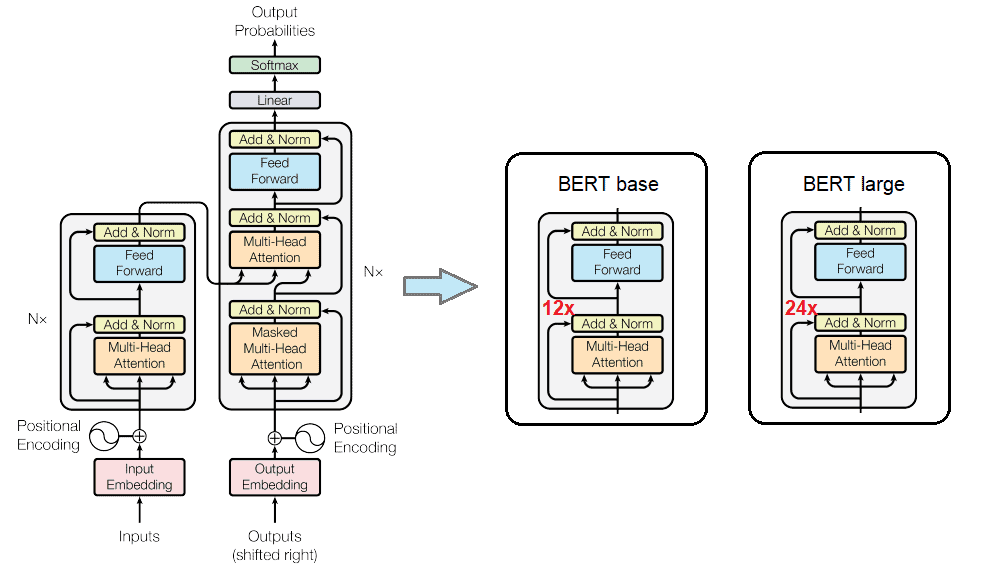
\includegraphics[width=\textwidth]{../../img/bert_base_large.jpg}
    \caption{Architettura di Transformers, BERT\textsubscript{BASE} e BERT\textsubscript{LARGE}}
    \label{fig:bert_input}
\end{figure}

Per ogni token in input, BERT calcola un embedding che è dato dalla somma di tre componenti come è possibile vedere in Figura \ref{fig:bert_embedding}:
\begin{itemize}
    \item \textbf{Token Embeddings}: sono i vettori di embedding per ciascun token nel vocabolario. Questi embedding sono allenati durante il pre-addestramento e sono aggiornati durante il fine-tuning. BERT utilizza una tecnica chiamata Wordpiece tokenization, in cui le parole vengono
    suddivise in sottostringhe più piccole chiamate wordpieces. Questa tecnica permette di
    creare un vocabolario flessibile contenente sia parole che sotto-parole, per esempio
    prefissi, suffissi o singoli caratteri. Il vocabolario così creato è in grado di gestire tutte le
    possibili sequenze di caratteri e di evitare l’utilizzo di token OOV (Out Of Vocabulary) \cite{WordPiece}.
    \item \textbf{Segment Embeddings}: sono i vettori di embedding che indicano a quale sequenza appartiene ciascun token. Questi embedding sono utilizzati per distinguere tra le due sequenze di input in un task di classificazione di sequenza.
    \item \textbf{Position Embeddings}: sono una componente critica per aiutare il modello a comprendere la posizione di ciascun token all’interno di una sequenza di testo. Questi embedding consentono a BERT di distinguere tra parole con lo stesso contenuto ma posizionate in posizioni diverse all’interno della frase. Ciò contribuisce a catturare le relazioni tra le parole in modo più completo e consente a BERT di eccellere in una vasta gamma di compiti di elaborazione del linguaggio naturale.
\end{itemize}

\begin{figure}[H]
    \centering
    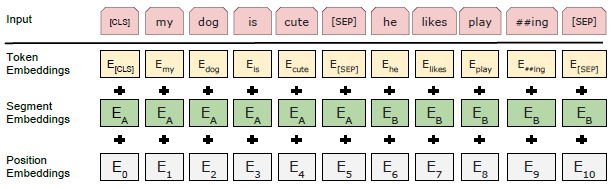
\includegraphics[width=\textwidth]{../../img/bert-input.png}
    \caption{Rappresentazione degli input di BERT}
    \label{fig:bert_embedding}
\end{figure}

\subsubsection{Pre-Training}
Il pre-training di BERT è stato effettuato usando due task di apprendimento non supervisionato: 
\begin{itemize}
    \item \textbf{Masked Language Model (MLM)}: in questo task venivano mascherate il 15\% dei token in input e si voleva far si che il modello predicesse i token mascherati. Questo processo in letteratura viene anche spesso chiamato \emph{Cloze} \cite{Taylor1953}. In questo caso i vettori dell'hidden layer finale che si riferisce al token mascherato venivano dati in input ad una funzione softmax sul vocabolario per predire il token mascherato. Per non creare troppo divario tra il pre-addestramento e il fine-tuning, durante questa fase di pre-training con MLM il token speciale [MASK] veniva utilizzato solo l'80\% delle volte, il 10\% delle volte veniva sostituito con un token casuale e il 10\% delle volte veniva lasciato il token originario.
    \item \textbf{Next Sentence Prediction (NSP)}: in molti task di NLP, come Question-Answering è necessario che i modelli siano in grado di comprendere relazioni tra due frasi. Per far si che il modello imparasse a riconoscere le relazioni tra frasi BERT è stato pre-addestrato su un task di predizione della frase successiva. Nello specifico, prese due frasi A e B il modello doveva predire se la frase B fosse la successiva rispetto alla frase A, questo nel dataset di training era vero nel 50\% dei casi. 
\end{itemize}

\subsubsection{Fine-tuning di BERT}

Il fine-tuning di BERT consiste nell'adattare il modello pre-allenato a compiti specifici, come la classificazione del testo, l'analisi del sentimento, il \textit{question answering} e altri. BERT utilizza l'architettura \textit{Transformer}, che permette di modellare relazioni complesse tra le parole di un testo grazie al meccanismo di \textit{self-attention}. Questo consente a BERT di processare sia singoli testi che coppie di testi.

Durante il fine-tuning, il modello pre-allenato viene ulteriormente addestrato su un dataset specifico del compito da risolvere, modificando tutti i parametri del modello. Questo include i pesi dei livelli di \textit{self-attention}, le rappresentazioni degli \textit{hidden layers} e i parametri degli strati di output. Ad esempio, per un compito di classificazione del testo, il token [CLS], che rappresenta l'intera sequenza, viene utilizzato per determinare la classe del testo. Per compiti a livello di token, come il \textit{named entity recognition} (NER), ogni token del testo viene etichettato individualmente.

Il processo di fine-tuning richiede meno risorse computazionali rispetto al pre-allenamento. Con l'uso di GPU o TPU, il fine-tuning può essere completato in poche ore, rendendo BERT un'opzione potente e versatile per una varietà di applicazioni di elaborazione del linguaggio naturale.

\subsection{DistilBERT}
Nel 2020 è stato presentato DistilBERT, un modello più piccolo e più veloce rispetto a BERT, sviluppato da Sanh et al. \cite{DistilBERT}. Il modello presentato dichiara che DistilBERT è in grado di ridurre la complessità di BERT del 40\% pur mantenendo il 97\% delle prestazioni di BERT ed essere 60\% più veloce. 

I risultati di DistilBERT sono stati ottenuti grazie ad una tecnica chiamata \emph{knowledge distillation}, che è una tecnica di compressione in cui modello più piccolo, detto \emph{modello studente}, è allenato per riprodurre i comportamenti di un modello più grande (o un insieme di modelli) detto \emph{modello insegnante}. Questo processo di distillazione permette di ridurre la complessità del modello studente, riducendo il numero di parametri e la complessità computazionale, mantenendo allo stesso tempo le prestazioni del modello più grande. Nell'apprendimento supervisionato, un modello di classificazione è generalmente allenato per predire l'istanza di una classi massimizzando la stima di probabilità di quella label. Un modello che funziona in maniera ottima predirrà una probabilità alta sulla classe corretta e probabilità vicine allo zero per le classi errate. 

Il training del modello student si basa su una combinazione di tecniche di distillazione del modello e di apprendimento supervisionato. Viene calcolata una  \textit{distillation loss} utilizzando le \textit{soft target probabilities} del modello insegnante. Questa perdita è definita come:

$$
L_{ce} = \sum_i t_i \log(s_i)
$$

dove $t_i$ (rispettivamente $s_i$) è una probabilità stimata dall'insegnante (rispettivamente dallo studente). Questa funzione obiettivo fornisce un segnale di training ricco sfruttando l'intera distribuzione dell'insegnante. Seguendo \cite{Hinton2015}, viene utilizzata una \textit{softmax-temperature}, definita come:

$$
p_i = \frac{\exp(z_i / T)}{\sum_j \exp(z_j / T)}
$$

dove $T$ controlla la morbidezza della distribuzione di output e $z_i$ è il punteggio del modello per la classe $i$. La stessa temperatura $T$ viene applicata sia allo studente che all'insegnante durante il training, mentre in fase di inferenza, $T$ è impostata a 1 per tornare ad una funzione \textit{softmax} standard.

L'obiettivo finale del training è una combinazione lineare della distillation loss $L_{ce}$ con la loss di  training supervisionato, cioè la loss del \textit{masked language modeling} $L_{mlm}$. Per allineare le direzioni dei vettori hidden state del modello student e teacher è stata aggiunta una  \textit{cosine embedding loss}, $L_{cos}$. La Loss finale è quindi definita come:
$$
L = \alpha L_{ce} + \beta L_{mlm} + \gamma L_{cos}
$$

Dove $\alpha$, $\beta$, e $\gamma$ sono pesi che bilanciano i diversi termini di loss. Questa combinazione permette di mantenere la qualità del modello distillato avvicinandolo il più possibile alla performance del modello insegnante.

\subsubsection{Architettura}
L'architettura del DistilBERT è simile a quella di BERT, ma con alcune differenze chiave. Vengono eliminati i \emph{token-type embedding} e la dimensione in termini di layer viene dimezzata. Sono state ottimizzate la maggior parte delle operazioni usate nell'architettura dei Transformer, come i \emph{linear layer} e \emph{layer normalisation} ed è stato dimostrato che ridurre la dimensione dell'hidden state non ha un impatto significativo sulle prestazioni del modello, quindi è rimasta invariata. Per l'inizializzazione del modello student è stato utilizzato un layer del modello BERT poichè hanno la stessa dimensione. 

\begin{figure}
    \centering
    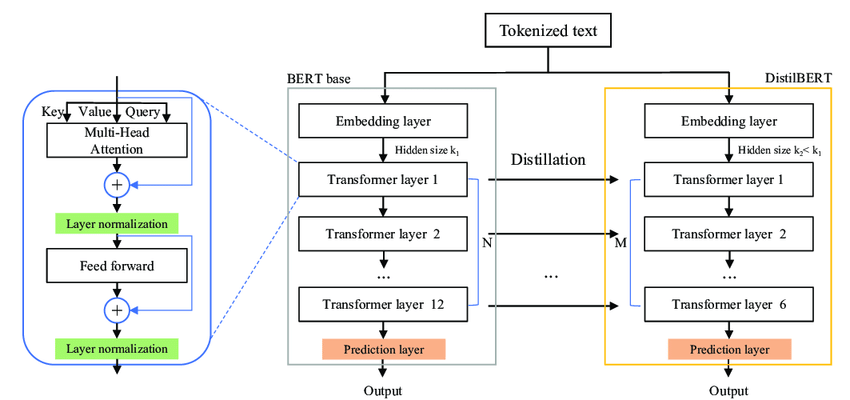
\includegraphics[width=\textwidth]{../../img/DistilBERT-Architecture.png}
    \caption{Architettura di DistilBERT}
    \label{fig:distilbert}
\end{figure}

\subsection{RoBERTa e CodeBERT}
A partire da BERT, nel 2019 è stato presentato RoBERTa (Robustly optimized BERT approach) da Liu et al. \cite{RoBERTa}. RoBERTa è un modello di deep learning pre-addestrato per l'elaborazione del linguaggio naturale, che migliora le prestazioni di BERT attraverso una serie di modifiche e ottimizzazioni. A livello architetturale, BERT e RoBERTa sono quasi identici, entrambi basati sull'architettura \textit{Transformer} con encoder bidirezionali. Tuttavia, le differenze principali tra i due risiedono nel processo di pre-training e nelle scelte di ottimizzazione. BERT utilizza due obiettivi di pre-training: il \textit{Masked Language Modeling} (MLM) e il \textit{Next Sentence Prediction} (NSP), mentre RoBERTa si concentra esclusivamente su MLM, eliminando l'obiettivo NSP. RoBERTa introduce anche il \textit{dynamic masking}, dove le maschere applicate ai token cambiano ad ogni epoca di training, rispetto al \textit{static masking} utilizzato da BERT. Inoltre, RoBERTa utilizza una quantità di dati di training molto più grande e adotta configurazioni di iperparametri più aggressive, come dimensioni del batch maggiori e tassi di apprendimento più elevati. Queste modifiche rendono RoBERTa più efficace e robusto, migliorando le sue performance su una varietà di compiti di elaborazione del linguaggio naturale rispetto a BERT.


Il modello CodeBERT è un modello presentato per la prima volta da Microsoft nel 2020 \cite{CodeBERT}. Il modello è stato costruito con la stessa architettura del modello RoBERTa-base, avendo quindi un numero totale di parametri pari a 125M. 

Nella fase di pretraining per questo modello l'input è stata una concatenazione di due segmenti: 

\section{Fase di Pre-Training di CodeBERT}

Nella fase di pre-training, l'input è costituito dalla concatenazione di due segmenti con un token separatore speciale, ovvero: $$[CLS], w_1, w_2, \ldots, w_n, [SEP], c_1, c_2, \ldots, c_m, [EOS]$$. Un segmento è testo in linguaggio naturale e l'altro è codice di un determinato linguaggio di programmazione. [CLS] è un token speciale posizionato all'inizio dei due segmenti, la cui rappresentazione nascosta finale viene considerata come la rappresentazione aggregata della sequenza per task di classificazione o ranking. Seguendo il metodo standard di elaborazione del testo nei \textit{Transformer}, è stato considerato un testo in linguaggio naturale come una sequenza di parole, splittandolo utilizzando in \textit{WordPiece}. Allo stesso modo, il codice sorgente è stato considerato come una sequenza di token.
L'output di CodeBERT offre: 
\begin{itemize}
    \item la rappresentazione vettoriale contestuale di ciascun token, sia per il linguaggio naturale che per il codice
    \item la rappresentazione di [CLS], che funziona come rappresentazione aggregata della sequenza, allo stesso modo che in BERT.
\end{itemize}
I dati di training che sono stati utilizzati nel pretraining sono sia dati \emph{bimodali}, ovvero dati che contengono sia testo scritto in linguaggio naturale che codice di un linguaggio di programmazione, che dati \emph{unimodali}, ovvero dati che contengono solo codice senza linguaggio naturale. 

I dati sono stati raccolti da repository Github, dove un datapoint:
\begin{itemize}
    \item \emph{bimodale:} è rappresentato da una singola funzione a cui è associata della documentazione in linguaggio naturale.
    \item \emph{unimodale:} è rappresentato da una singola funzione senza documentazione in 
    linguaggio naturale.
\end{itemize}
Nello specifico, è stato utilizzato un dataset offerto da \cite{CodeBERTDataset} che contiene 2.1M di dati bimodali e 6.4M di dati unimodali suddivisi in 6 linguaggi di programmazione: Python, Java, JavaScript, Ruby, Go e PHP. Tutti i dati erano provenienti da repository pubblici e open-source su Github e sono stati filtrati sulla base cinque criteri:
\begin{enumerate}
    \item ogni progetto deve essere usato da almeno un altro progetto 
    \item ogni documentazione viene troncata al primo paragrafo
    \item le documentazioni inferiori a tre token sono state rimosse
    \item funzioni piu corte di tre linee di codice sono state rimosse
    \item le funzioni che abbiamo nel nome la sottostringa "test" sono state rimosse
\end{enumerate}

Il pretraining di è stato effettuato utilizzando due diverse funzioni obiettivo. Il primo metodo è stato il MLM, che è stato utilizzato per preaddestrare il modello a predire i token mascherati, questo è stato applicato sui dati bimodali. Anche in questo caso, seguendo l'approccio usato dal modello BERT originario \cite{BERT},  sono stati mascherati il 15\% dei token tra token appartenenti al linguaggio naturale e token facenti parte del codice sorgente. Il secondo metodo applicato è stato il \emph{replaced token detection} che utilizza sia i dati bimodati che quelli unimodali.  Durante il pre-training, alcuni token nell'input originale, che può essere testo in linguaggio naturale o codice, vengono sostituiti con token casuali. Il compito del modello è quindi rilevare quali token sono stati sostituiti. Il processo funziona nel seguente modo: il modello riceve una sequenza di token contenente sia token originali che token sostituiti. Per ogni token, il modello deve prevedere una probabilità che indichi se il token è stato sostituito o meno. L'obiettivo di training per RTD è minimizzare la perdita di classificazione binaria tra i token originali e quelli sostituiti. Questo metodo sfrutta l'intero contesto della sequenza, permettendo a CodeBERT di apprendere rappresentazioni più ricche e accurate sia per il linguaggio naturale che per il codice.

Per quanto riguarda il fine-tuning, allo stesso modo di BERT, CodeBERT può essere specializzato su task specifici tunando tutti i suoi parametri in modo molto efficiente. Il modello ha ottenuto performance allo stato dell'arte per task che includono ricerca di codice tramite linguaggio naturale, generazione di documentazione a partire dal codice. 


\section{Implementazione}
I tre modelli precedenti, BERT, DistilBERT e CodeBERT sono quelli scelti ed utilizzati in questo lavoro per la classificazione di vulnerabilità degli smart contracts. I task di classificazione possono dividersi in tre categorie principali: 
\begin{itemize}
    \item \textbf{Classificazione Binaria:} in cui il modello deve predire se un dato elemento appartiene o meno ad una classe specifica. Facendo un esempio nel contesto degli smart contracts, un task di classificazione binaria comporterebbe la predizione della presenza o meno di vulnerabilità in uno smart contract. 
    \item \textbf{Classificazione Multiclasse:} in cui il modello deve predire, all'interno di un insieme di classi, a quale classe appartiene un dato elemento, posto che possa appartenere ad una sola classe. Ad esempio, un task di classificazione multiclasse potrebbe essere quello di prevedere la vulnerabilità presente in uno smart contract posto che questo possa avere un solo tipo di vulnerabilità.
    \item \textbf{Classificazione Multilabel:} in cui il modello deve predire, all'interno di un insieme di classi, a quali classi appartiene un dato elemento, posto che possa appartenere a più classi contemporaneamente. 
\end{itemize}
Questo lavoro è stato affrontato come un task di classificazione multilabel, in quanto uno smart contract può avere più di una vulnerabilità contemporaneamente. 

Il codice per il pre-processing dei dati, la costruzione, il training e la valutazione dei modelli è stato scritto in Python. Python è un linguaggio di programmazione Touring-completo ad alto livello, ampiamente riconosciuto per la sua semplicità e leggibilità. La vasta disponibilità di librerie e strumenti specifici per l'elaborazione del linguaggio naturale e l'apprendimento automatico, come NumPy, Pandas e Scikit-learn, rende Python una scelta ideale per questo tipo di ricerca. Inoltre, Python è supportato da una vasta comunità di sviluppatori e ricercatori, che lo rendono uno dei linguaggi più utilizzati a livello mondiale per la manipolazione di dati e per lo sviluppo di modelli di Machine e Deep Learning. In aiuto a Python è stata utilizzata la libreria PyTorch,  una libreria di deep learning altamente performante e flessibile, sviluppata da Facebook AI Research (FAIR) \cite{Pytorch}. PyTorch offre un'interfaccia intuitiva e dinamica per la costruzione e l'addestramento di modelli di apprendimento profondo, facilitando la sperimentazione e l'ottimizzazione dei modelli. Inoltre, PyTorch è supportato da una comunità di ricerca attiva e in crescita, che contribuisce con numerosi modelli pre-addestrati e risorse che accelerano lo sviluppo e la valutazione dei modelli. Queste caratteristiche rendono Python e PyTorch l'ovvia scelta per questo lavoro.

Fondamentali per lo sviluppo sono state altre due librerie offerte da HuggingFace, rispettivamente Transformers e Datasets. Transformers è una libreria open-source che offre un'implementazione di modelli di apprendimento profondo pre-addestrati, tra cui BERT, RoBERTa, DistilBERT e molti altri. Questa libreria offre un'interfaccia semplice e intuitiva per caricare, costruire e addestrare modelli di apprendimento profondo, facilitando la sperimentazione e l'ottimizzazione dei modelli. Datasets, invece, è una libreria open-source che offre un'interfaccia semplice e intuitiva per caricare e manipolare dataset che sono stati caricati sulla piattaforma HuggingFace. Questa libreria offre una vasta gamma di dataset pre-caricati, tra cui il dataset \textit{rossini2022slitherauditedcontracts} utilizzato in questo lavoro, semplificando il processo di raccolta dei dati. 

Di seguito, verranno presentati tutti gli esperimenti effettuati e i vari modelli costruiti, i cui risultati verranno poi discussi nel capitolo \ref{chap:results} successivo.

\subsection{BERT-base}
Il primo modello ricostruito è stato un modello BERT base. Il modello pretrainato a cui si è fatto riferimento è stato \textit{bert-base-uncased}, un modello BERT base pre-addestrato su un corpus di testo in lingua inglese. Dopo essere stato caricato il modello ne viene estratto il pooling output per il primo token, il token [CLS] che come descritto nella sezione \ref{sec:bert} è utilizzato come rappresentazione aggregata della sequenza per task di classificazione. Questo output viene poi passato ad un layer di classificazione lineare, che prende in input un vettore di dimensione pari all'hidden state di BERT, quindi 768, e restitusce un vettore di output con dimensione pari al numero di classi (nel nostro caso 5). Questo vettore di output viene poi passato ad una funzione di attivazione softmax, che restituisce una distribuzione di probabilità su tutte le classi. Questo modello viene utilizzato per la classificazione sia del codice sorgente che del bytecode dei contratti. Mostriamo ora un esempio di codice per la costruzione del modello: 
\begin{python}
    class BERTClassifier(torch.nn.Module):
    def __init__(self):
        super(BERTClassifier, self).__init__()
        self.bert_model = transformers.BertModel.from_pretrained('bert-base-uncased')
        self.dropout = torch.nn.Dropout(0.3)
        self.linear = torch.nn.Linear(768, NUM_CLASSES)
    
    def forward(self, input_ids, attention_mask, token_type_ids):
        _, pooled_output = self.bert_model(input_ids, attention_mask=attention_mask, token_type_ids=token_type_ids, return_dict=False)
        dropout_output = self.dropout(pooled_output)
        linear_output = self.linear(dropout_output)
        return linear_output
\end{python}
Il \emph{pooled\_output} è la rappresentazione vettoriale estratta dal modello BERT che rappresenta un'aggregazione delle informazioni apprese dal testo di input. Questa rappresentazione viene ottenuta tramite un processo di "pooling" delle rappresentazioni dei token di input prodotte dal modello BERT.
Il layer di Dropout è stato aggiunto per evitare l'overfitting del modello. Il modello è stato addestrato utilizzando l'ottimizzatore Adam con un learning rate di $1 \times 10^{-5}$ e una dimensione del batch di 8.
\subsubsection{Loss Function}
La funzione di loss scelta è stata la BCEWithLogitsLoss, che è stata utilizzata per la classificazione multilabel. 
La funzione di perdita \textit{BCEWithLogitsLoss} è una combinazione efficiente della \textit{Binary Cross Entropy} (BCE) e di una funzione logistica di attivazione, spesso utilizzata per compiti di classificazione binaria in reti neurali. Questa funzione di loss applica un'attivazione sigmoide ad una Binary Cross Entropy. 
$$
\ell(x, y) = L = \begin{bmatrix} l_1, \ldots, l_N \end{bmatrix}^\top, \quad l_n = -w_n \left[ y_n \cdot \log \sigma(x_n) + (1 - y_n) \cdot \log (1 - \sigma(x_n)) \right],
$$

\subsection{DistilBERT}
La costruzione di un modello DistilBERT avviene in modo pressochè identico a quello del modello BERT. Anche in questo caso si è utilizzato il modello pre-addestrato \textit{distilbert-base-uncased}, proveniente dalla libreria Transformers. Mostriamo ora il codice per la costruzione del modello:
\begin{python}
    class DistilBERTClass(torch.nn.Module):
    def __init__(self, NUM_CLASSES):
        super(DistilBERTClass, self).__init__()
        self.num_classes = NUM_CLASSES
        self.distilbert = DistilBertModel.from_pretrained('distilbert-base-uncased')
        self.dropout = torch.nn.Dropout(0.3)
        self.fc = torch.nn.Linear(768, NUM_CLASSES)
    
    def forward(self, input_ids, attention_mask):
        outputs = self.distilbert(input_ids=input_ids, attention_mask=attention_mask)
        pooled_output = outputs.last_hidden_state[:, 0]
        pooled_output = self.dropout(pooled_output)
        output = self.fc(pooled_output)
        return output
\end{python}
Anche in questo caso, il modello è stato addestrato utilizzando l'ottimizzatore Adam con un learning rate di $1 \times 10^{-5}$ e una dimensione del batch di 8 e la funzione di loss BCEWithLogitsLoss. Come per il modello BERT, il layer di Dropout è stato aggiunto per evitare l'overfitting del modello.

Come si può notare dal codice sopra riportato, a differenza del modello BERT, il modello DistilBERT non prende in input i token type ids, in quanto non sono presenti nella struttura del modello DistilBERT.

\subsection{CodeBERT}
Anche il modello CodeBERT è stato costruito in modo simile ai modelli BERT e DistilBERT. Il modello pre-addestrato utilizzato è stato \textit{microsoft/codebert-base}, proveniente dalla libreria Transformers. Mostriamo ora il codice per la costruzione del modello:
\begin{python}
    class CodeBERTClass(torch.nn.Module):
        def __init__(self, NUM_CLASSES):
            super(CodeBERTClass, self).__init__()
            self.num_classes = NUM_CLASSES
            self.codebert = AutoModel.from_pretrained('microsoft/codebert-base')
            self.dropout = torch.nn.Dropout(0.3)
            self.fc = torch.nn.Linear(768, NUM_CLASSES)
        
        def forward(self, ids, mask):
            outputs = self.codebert(input_ids=ids, attention_mask=mask)
            pooled_output = outputs.pooler_output
            pooled_output = self.dropout(pooled_output)
            output = self.fc(pooled_output)
            return output
\end{python}
Anche in questo caso, il modello è stato addestrato utilizzando l'ottimizzatore Adam con un learning rate di $1 \times 10^{-5}$ e una dimensione del batch di 8 e la funzione di loss BCEWithLogitsLoss. Come per i modelli BERT e DistilBERT, il layer di Dropout è stato aggiunto per evitare l'overfitting del modello.

\subsection{CodeBERT con aggregazione}
Uno dei problemi principali riscontrati nel training dei precedenti modelli è i modelli della famiglia BERT hanno una capacità massima in input di 512 token. I nostri smart contract, come visto precedentemente hanno una lunghezza media di circa 1500 token, dare quindi in input al modello solo 512 token significa far si che il modello analizzi, in molti casi, solo una piccola porzione iniziale dei nostri contratti. Per ovviare a questo problema, è stato deciso di dividere i nostri contratti in sotto-contratti di lunghezza massima 512 token e poi aggregare gli embedding prodotti da CodeBERT per ogni sotto-contratto tramite delle funzioni di aggregazione come media e massimo. Questo approccio permette di far si che il modello possa analizzare l'intero contratto, anche se in sotto-parti. Mostriamo ora il codice per la costruzione del modello: 
\begin{python}
    class CodeBERTAggregatedClass(torch.nn.Module):
        def __init__(self, num_classes, aggregation='mean', dropout=0.3):
            super(CodeBERTAggregatedClass, self).__init__()
            self.codebert = AutoModel.from_pretrained('microsoft/codebert-base', cache_dir="./cache")
            self.dropout = torch.nn.Dropout(dropout)
            self.fc = torch.nn.Linear(self.codebert.config.hidden_size, num_classes)
            self.aggregation = aggregation

        def forward(self, input_ids, attention_masks):
            batch_size, seq_len = input_ids.size()

            # Divide input_ids e attention_masks in blocchi di 512 token
            num_chunks = (seq_len + 511) // 512
            input_ids = input_ids[:, :512*num_chunks].view(batch_size * num_chunks, 512)
            attention_masks = attention_masks[:, :512*num_chunks].view(batch_size * num_chunks, 512)

            outputs = self.codebert(input_ids=input_ids, attention_mask=attention_masks)

            last_hidden_states = outputs.last_hidden_state
            cls_tokens = last_hidden_states[:, 0, :]

            cls_tokens = cls_tokens.view(batch_size, num_chunks, -1)

            if self.aggregation == 'mean':
                aggregated_output = torch.mean(cls_tokens, dim=1)
            elif self.aggregation == 'max':
                aggregated_output, _ = torch.max(cls_tokens, dim=1)
            else:
                raise ValueError("Aggregation must be 'mean' or 'max'")

            aggregated_output = self.dropout(aggregated_output)
            output = self.fc(aggregated_output)
            return output
\end{python}
Questo approccio è stato testato sia con la funzione di aggregazione \emph{mean} che con la funzione di aggregazione \emph{max}, che restituiscono rispettivamente la media e il massimo degli embedding prodotti da CodeBERT per ogni sotto-contratto. Inoltre, sono stati testati aprrocci per entrambi in cui venivano utilizzati due o tre blocchi di codice, quindi si classificavano rispettivamente 1024 e 1536 token.
\subsection{CodeBert con concatenazione}
Un altro approccio complementare alla risoluzione del problema legato al massimo numero di token che i modelli della famiglia BERT possono accettare come input è stato quello di concatenare gli embedding prodotti da CodeBERT per ogni sotto-contratto. Questo approccio permette di mantenere l'informazione relativa a tutti i token del contratto e di fornire al modello un'informazione più completa. Mostriamo ora il codice per la costruzione del modello:
\begin{python}
    class CodeBERTConcatenatedClass(torch.nn.Module):
    def __init__(self, num_classes, dropout=0.3):
        super(CodeBERTConcatenatedClass, self).__init__()
        self.codebert = AutoModel.from_pretrained('microsoft/codebert-base', cache_dir="./cache")
        self.dropout = torch.nn.Dropout(dropout)
        # Multiply hidden_size by the number of chunks you're concatenating
        self.fc = torch.nn.Linear(self.codebert.config.hidden_size * CODE_BLOCKS, num_classes)

    def forward(self, input_ids, attention_masks):
        batch_size, seq_len = input_ids.size()

        # Divide input_ids and attention_masks into chunks of 512 tokens
        num_chunks = (seq_len + 511) // 512
        input_ids = input_ids[:, :512*num_chunks].reshape(batch_size * num_chunks, 512)
        attention_masks = attention_masks[:, :512*num_chunks].reshape(batch_size * num_chunks, 512)

        outputs = self.codebert(input_ids=input_ids, attention_mask=attention_masks)

        last_hidden_states = outputs.last_hidden_state
        cls_tokens = last_hidden_states[:, 0, :]

        # Concatenate the CLS tokens of the various chunks
        cls_tokens = cls_tokens.reshape(batch_size, num_chunks, -1)
        concatenated_output = cls_tokens.reshape(batch_size, -1)

        concatenated_output = self.dropout(concatenated_output)
        output = self.fc(concatenated_output)
        return output
\end{python}
In questo caso, si divide la stringa in input in chunk da 512 token e si ottengono gli embedding prodotti da codeBERT per ognuno di questi chunk. Questi embedding vengono poi concatenati e passati ad un layer di classificazione lineare. Anche in questo caso l'approccio è stato testato sia con due che con tre blocchi di codice, quindi si classificavano rispettivamente 1024 e 1536 token. 
\subsection{Train e Validation}
Tutti i modelli sono stati addestrati (o fine-tunati) per 20 epoche, con un learning rate di $1 \times 10^{-5}$. Per evitare l'overfitting, è stato utilizzato un layer di Dropout con un rate del 30\%. La funzione di loss utilizzata è stata la BCEWithLogitsLoss, che è stata utilizzata per la classificazione multilabel. L'ottimizzatore utilizzato è stato Adam. I modelli sono stati addestrati su una GPU NVIDIA 2080Ti. A seguito di limitazioni dovute alla potenza di calcolo e alla grandezza del dataset in alcuni casi è stato necessario ridurre la batch size. Nello specifico, per i modelli di aggregazione e concatenazione che utilizzavano due blocchi di codice (1024 token) la batch size è stata ridotta a 4, mentre per i modelli che utilizzavano tre blocchi di codice (1536 token) la batch size è stata ridotta a 2. Questa potrebbe essere sicuramente una limitazione al lavoro, in quanto una batch size ridotta potrebbe portare ad un addestramento più lento e a risultati meno accurati. Si rimanda a futura ricerca la possibilità di addestrare i modelli con potenze di calcolo maggiori per effettuare dei tuning dei parametri più accurati. 

\section{Gemini}
Gemini è un 
\end{document}
